\section{Ахова працы}

\subsection{Арганізацыя сістэмы кіравання аховай працы на прадпрыемстве}

Сістэма кіравання аховай працы (АП) у замежным таварыстве з абмежаванай адказнасцю «ЭПАМ Сістэмз», прызначана для прадухілення траўм і захворванняў, звязаных з вытворчай дзейнасцю, а таксама для абароны і ўмацавання здароўя супрацоўнікаў арганізацыі; яна таксама накіравана на паляпшэнне ўмоў працы і навакольнага асяроддзя.

На малюнку \ref{img: epam healthy system} прадстаўлена структура службы аховы працы ў арганізацыі «ЭПАМ Сістэмз».

\begin{figure}[h!]
    \centering
    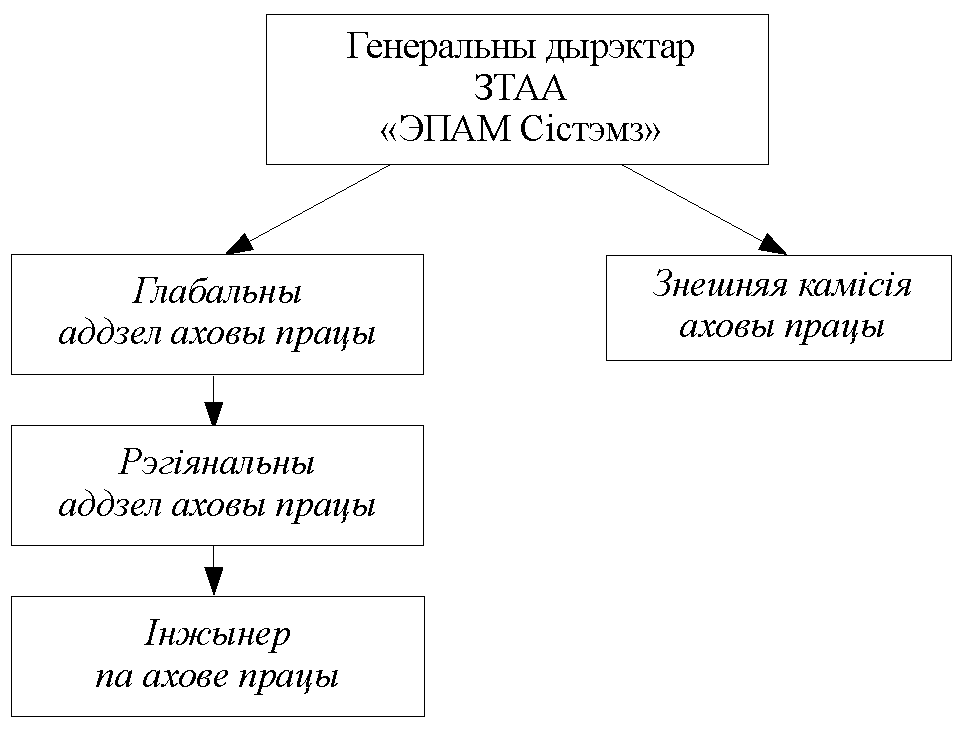
\includegraphics[width=0.7\textwidth]{epam_healthy_system.pdf}
    \caption{Структура службы аховы працы ў арганізацыі}
    \label{img: epam healthy system} 
\end{figure}

Штогод, у мэтах далейшага ўдасканалення арганізацыі работ па АП і забеспячэння выканання заканадаўства аб АП, генеральны дырэктар сцвярджае план мерапрыемстваў, складзены дырэктарам адміністрацыйнага дэпартамента і начальнікам глабальнага аддзела АП, якi ўключае:
\begin{enumerate}
    \item удасканаленне дакументацыі па АП, неабходнай у арганізацыі, ўкараненне перадавога досведу і навуковых распрацовак па АП і ТБ у арганізацыі;
    \item правядзенне папярэдніх медыцынскіх аглядаў, кансультацыі з дактарамі вузкіх спецыялізацый і вакцынацыя супрацоўнікаў перад прагназуемымі перыядамі эпідэміялагічных захворванняў;
    \item набыццё мыйных сродкаў і сродкаў асабістай гігіены для супрацоўнікаў арганізацыі, закупка сродкаў індывідуальнай абароны;
    \item арганізацыя правядзення лабараторна-інструментальных даследаванняў фактараў вытворчага асяроддзя на працоўных месцах у арандаваных памяшканнях;
    \item ажыццяўленне кантролю за правядзеннем перыядычных (паўторных) інструктажоў па АП і пажарнай бяспекі (ПБ) у вытворчых падраздзяленнях арганізацыі;
    \item выяўленне вытворчых небяспекі з мэтай кіравання (зніжэння) рызык перадумоў стварэння сітуацый, якія прыводзяць да няшчасных выпадкаў;
    \item забеспячэнне тэхнічна абгрунтаваных умоў эксплуатацыі сістэм вентыляцыі і кандыцыянавання, а таксама абследаванне і кантроль за станам апорных канструкцый будынкаў.
\end{enumerate}

Кіраўнікі дэпартаментаў арганізацыі павінны быць азнаёмлены з загадам аб зацвярджэнні плана мерапрыемстваў па АП, пры гэтым кантроль за выкананнем загаду ускладаецца на дырэктара адміністрацыйнага дэпартамента.

Чаканая сацыяльная эфектыўнасць ад увядзення мерапрыемстваў па АП:
\begin{enumerate}
    \item зніжэнне імавернасці ўзнікнення траўманебяспечных сiтуацый;
    \item падтрыманне умоў працы на працоўных месцах арганізацыі ў адпаведнасці з санітарна-гігіенічнымі нормамі;
    \item паляпшэнне ўмоў навучання, правядзення інструктажоў у арганізацыі;
    \item фарміраванне нарматыўнай базы ў арганізацыі;
    \item зніжэнне рызык ўзнікнення агульных захворванняў;
    \item маніторынг умоў працы на працоўных месцах арганізацыі.
\end{enumerate}

Інжынер па ахове працы, у адпаведнасці са сваімі паўнамоцтвамі, мае права:
\begin{enumerate}
    \item праводзіць праверкі выканання патрабаванняў па АП, стану ўмоў працы;
    \item запытваць і атрымліваць неабходную інфармацыю па пытаннях АП, патрабаваць пісьмовыя тлумачэнні ад службовых асоб, якія працуюць і якія дапусцілі парушэнні патрабаванняў па АП;
    \item прыпыняць ва ўстаноўленым заканадаўствам парадку эксплуатацыю абсталявання, інструмента, прыстасаванняў, транспартных сродкаў, выкананне работ (аказанне паслуг) пры выяўленні парушэнняў, якія ствараюць пагрозу для жыцця або здароўя супрацоўнікаў і навакольных, да іх ліквідацыі;
    \item уносіць прапановы па паляпшэнню ўмоў працы супрацоўнікаў, папярэджваючы вытворчы траўматызм і прафесійныя захворванні.
\end{enumerate}

Такім чынам, асноўнымі задачамі службы аховы працы ў арганізацыі з'яўляюцца:
\begin{enumerate}
    \item арганізацыя навучання і праверкі ведаў супрацоўнікаў па пытаннях аховы працы;
    \item арганізацыя і каардынацыя мерапрыемстваў па ахове працы ў арганізацыі;
    \item кантроль за выкананнем патрабаванняў па АП;
    \item удасканаленне ўмоў працы і правядзенне прафілактычных работ па папярэджанні вытворчага траўматызму, прафесійных і вытворча абумоўленых захворванняў.
\end{enumerate}
